\documentclass[11pt,letterpaper]{article}

\usepackage[
  letterpaper,
  left=0.6in,
  right=0.6in,
  top=0.8in,
  bottom=0.8in,
  headheight=14pt,
  headsep=0.25in,
  footskip=0.35in
]{geometry}

\usepackage{fontspec}
\setmainfont{Google Sans}
\usepackage{microtype}

\usepackage{amsmath}
\usepackage{amssymb}
\usepackage{booktabs}
\usepackage{array}
\usepackage{multirow}
\usepackage{tabularx}
\usepackage{graphicx}
\usepackage{caption}
\usepackage{enumitem}
\usepackage[section]{placeins}
\usepackage[hidelinks]{hyperref}
\usepackage{tikz}
\usetikzlibrary{fit,positioning,calc,arrows.meta}
\usepackage{xcolor}
\usepackage{float}
\usepackage{needspace}
\renewcommand{\topfraction}{0.9}
\renewcommand{\floatpagefraction}{0.8}

\graphicspath{{figures/}}
\captionsetup{font=small,labelfont=bf,labelsep=period,skip=6pt}
\setlist[itemize]{leftmargin=1.2em,itemsep=2pt,topsep=3pt,parsep=0pt}
\setlist[enumerate]{leftmargin=1.4em,itemsep=2pt,topsep=3pt,parsep=0pt}
\setlength{\parskip}{4pt}
\setlength{\emergencystretch}{2em}

\pagestyle{plain}

\setlength{\parindent}{0pt}

\newcommand{\todo}[1]{\textcolor{red}{\textbf{[#1]}}}
\newcommand{\taskbanner}[2]{\begin{center}{\small\bfseries #1}\\[3pt]{\Large\bfseries #2}\end{center}\vspace{2pt}\hrule\vspace{8pt}}

\begin{document}

\begin{center}
  {\small\bfseries AI651: Deep Learning for Space, Time and Graphs}\\[6pt]
  {\Large\bfseries Assignment 3}\\[6pt]
\end{center}

\vspace{2pt}
\noindent\begin{tabular}{@{}p{0.8in}p{5.6in}@{}}
\textbf{Name}      & Muhammad Hussain Habib \\
\textbf{Roll no.}  & 27100016 \\
\textbf{Repository} & \texttt{https://github.com/Hussain004/DL4STG-PA3} \\
\end{tabular}

\vspace{6pt}
\normalsize

\taskbanner{Question 1}{What does a sum remember?}

A GNN layer only gets to see a summary of each neighbourhood, so this question is about
what can and cannot survive that summary. The question has three parts. First, an affine
message, which turns out to remember only two numbers about the neighbourhood, no matter
what $w$, $c$ or $\rho$ are. Second, a nonlinear scalar message that is allowed to be anything,
which can remember everything, if it is allowed a large enough number to write it in. Third,
the three standard aggregators with one-hot messages, where the aggregator (not the message)
decides what the layer can compute. The crux throughout is the same: whatever the aggregate
throws away, no choice of readout $\rho$ can bring back. Every numerical claim below is
checked by \texttt{q1/code/verify\_encodings.py}.

\section*{(a) The affine message: two numbers survive}

The layer computes
\begin{equation*}
h_v \;=\; \rho\Bigl(\sum_{u \in N(v)} \phi(x_u)\Bigr),
\qquad \phi(x) = wx + c .
\end{equation*}
Writing out the sum,
\begin{equation*}
\sum_{u \in N(v)} (w x_u + c)
\;=\;
w \sum_{u \in N(v)} x_u \;+\; c \sum_{u \in N(v)} 1
\;=\;
w S_v + c\, n_v ,
\end{equation*}
where $S_v = \sum_{u \in N(v)} x_u$ and $n_v = |N(v)|$. So the whole neighbourhood reaches
$\rho$ as the single number $w S_v + c\, n_v$, and
\begin{equation*}
h_v \;=\; \rho\bigl(w S_v + c\, n_v\bigr).
\end{equation*}

If two neighbourhoods have the same $n_v$ and the same $S_v$, then for every choice of $w$ and
$c$ this scalar is the same number. Since $\rho$ receives nothing else, its output is the same
number too. A nonlinear $\rho$ does not help: it can be an arbitrarily complicated function,
but it is a function \emph{of} $w S_v + c\, n_v$, and identical inputs give identical outputs.
The failure is upstream of $\rho$, in the aggregate, which is why the aggregate has to be the
thing that carries the information.

Two such neighbourhoods with different numbers of steady neighbours:
\begin{equation*}
N_1 = \{-1,\, 0,\, +1\}, \qquad N_2 = \{0,\, 0,\, 0\}.
\end{equation*}
Both have $n_v = 3$ and $S_v = 0$, so they are indistinguishable to the layer: with $w = 2$,
$c = 1$ the aggregate is $2 \cdot 0 + 1 \cdot 3 = 3$ in both cases, and it is equal for any
other $w$ and $c$ too. But $N_1$ has one steady neighbour and $N_2$ has three, so the number of
steady neighbours, and for that matter the whole distribution of trends, is genuinely
different information that the affine aggregate cannot see. There are infinitely many such
pairs: whenever a neighbourhood contains a slowing/speeding pair $\{-1, +1\}$ (which
contributes $0$ to $S_v$), replacing that pair by two steady neighbours leaves both $n_v$ and
$S_v$ unchanged, while the steady count increases by two.

What the affine message passes on is therefore exactly two things, the size of the
neighbourhood and the total trend, and everything else about the neighbourhood is gone before
$\rho$ runs.

\section*{(b) A nonlinear message in one number: place values}

Now $\phi$ may be any function, still producing a single number.
Writing the counts as $a$ (slowing), $b$ (steady), $c$ (speeding up), so that $a + b + c = n_v$
and $S_v = c - a$. We suppose $1 \le |N(v)| \le K$ with $K$ known. Then $0 \le a, b, c \le K$.

Take a base $B$ and let the sum read the counts as digits of one number:
\begin{equation*}
\phi(-1) = 1, \qquad \phi(0) = B, \qquad \phi(+1) = B^2 .
\end{equation*}
Then the sum over the neighbourhood is
\begin{equation*}
m \;=\; a \cdot 1 + b \cdot B + c \cdot B^2,
\end{equation*}
which is exactly the base-$B$ number with digits $(c, b, a)$. The counts come back out as
\begin{equation*}
a = m \bmod B, \qquad
b = \Bigl\lfloor \frac{m}{B} \Bigr\rfloor \bmod B, \qquad
c = \Bigl\lfloor \frac{m}{B^2} \Bigr\rfloor .
\end{equation*}

{The base must be at least $K + 1$.} Each count can be as large as $K$, and a digit is
only unambiguous if it is smaller than its base. With $B = K$ a count of $K$ is the
same digit as $0$ with a carry into the next position, which collapses distinct triples: for
$K = 8$ with $B = 8$, the neighbourhoods with counts $(8, 0, 0)$ and $(0, 1, 0)$ both give
$m = 8$. With $B = K + 1$ no carry can ever happen, since $a, b, c \le K < B$, and the three
digits are read off independently.

For $K = 8$ this gives $B = 9$ and
\begin{equation*}
\phi(-1) = 1, \qquad \phi(0) = 9, \qquad \phi(+1) = 81, \qquad
m = a + 9 b + 81 c .
\end{equation*}
The largest value $m$ can take is $8 + 8 \cdot 9 + 8 \cdot 81 = 728 < 9^3 = 729$, so everything
fits in three base-9 digits. As a worked example, the neighbourhood $\{-1, 0, +1, +1\}$ has
$(a, b, c) = (1, 1, 2)$, giving $m = 1 + 9 + 2 \cdot 81 = 172$; decoding, $172 \bmod 9 = 1$,
$\lfloor 172 / 9 \rfloor \bmod 9 = 19 \bmod 9 = 1$, and $\lfloor 172 / 81 \rfloor = 2$, so the
counts $(1, 1, 2)$ come back exactly.

I verified the construction in NumPy on every possible triple with $1 \le a + b + c \le K$:
for $K = 8$ there are $\binom{11}{3} - 1 = 164$ such triples and all 164 decode exactly, and
the same check passes for every $K$ from $1$ to $16$ (\texttt{q1/results/verify\_encodings.json}). This is a construction about representability, not
about learnability: $m$ has magnitude up to roughly $K^3$, which is fine for an exact
arithmetic argument and says nothing about what a small MLP with floating point would
actually learn.

For the simpler target in one number part. If all that is wanted is the number of non-steady
neighbours (either $-1$ or $+1$), there is nothing to encode and one multiplication does it:
\begin{equation*}
\phi(x) = x^2 \quad\Longrightarrow\quad
\phi(-1) = \phi(+1) = 1, \;\; \phi(0) = 0, \quad\text{so}\quad
\sum_{u \in N(v)} \phi(x_u) = a + c .
\end{equation*}
This works for every neighbourhood size, with no base to choose and no assumption on $K$.

\section*{(c) Sum, mean and max with one-hot messages}

For this part the message is fixed as the one-hot vector
$\phi(-1) = (1,0,0)$, $\phi(0) = (0,1,0)$, $\phi(+1) = (0,0,1)$, with coordinates
(slowing, steady, speeding up). A neighbourhood with counts $(a, b, c)$ and size $n_v$ then
produces
\begin{align*}
\text{sum}  &:\; (a,\; b,\; c), \\
\text{mean} &:\; \Bigl(\tfrac{a}{n_v},\; \tfrac{b}{n_v},\; \tfrac{c}{n_v}\Bigr), \\
\text{max}  &:\; \bigl(\mathbf{1}[a > 0],\; \mathbf{1}[b > 0],\; \mathbf{1}[c > 0]\bigr).
\end{align*}
The readout $\rho$ sees only the aggregated vector: it is not told $n_v$. Sum keeps the exact
counts, mean keeps only the proportions, and max keeps only whether each trend appeared at
all.

\begin{table}[htbp]
\centering
\footnotesize
\setlength{\tabcolsep}{5pt}
\renewcommand{\arraystretch}{0.92}
\begin{tabularx}{\textwidth}{@{}p{0.78in}p{0.52in}p{0.62in}X@{}}
\toprule
\textbf{Task} & \textbf{Method} & \textbf{Possible?} & \textbf{Reason} \\
\midrule
\multirow{3}{0.78in}{(i) Count steady neighbours}
 & Sum   & Yes & Read the second coordinate, which is exactly $b$. Any function $\rho$ that returns
                   it computes the count. \\
 \cmidrule{2-4}
 & Mean  & No  & The second coordinate is $b / n_v$, and $\rho$ is not told $n_v$. $N_1 = \{0\}$ and
                  $N_2 = \{0, 0\}$ both give $(0, 1, 0)$, but the counts are $b = 1$ and $b = 2$. \\
 \cmidrule{2-4}
 & Max   & No  & The second coordinate is $\mathbf{1}[b > 0]$, presence only. The same pair $N_1 = \{0\}$
                  and $N_2 = \{0, 0\}$ both give $(0, 1, 0)$, but $b = 1$ and $b = 2$. \\
\midrule
\multirow{3}{0.78in}{(ii) More than half of the neighbours are slowing}
 & Sum   & Yes & $\rho$ has $(a, b, c)$, hence $n_v = a + b + c$. Answer \emph{yes} exactly when
                 $2a > n_v$, i.e. $a > b + c$. \\
 \cmidrule{2-4}
 & Mean  & Yes & The first coordinate is $a / n_v$. Answer \emph{yes} exactly when the first coordinate
                 exceeds $1/2$; $n_v$ is not needed separately. \\
 \cmidrule{2-4}
 & Max   & No  & $N_1 = \{-1, -1, 0\}$ gives $(2, 1, 0)$ (a majority are slowing, $2 > 3/2$) and
                 $N_2 = \{-1, 0, 0\}$ gives $(1, 2, 0)$ (not a majority, $1 < 3/2$). Both give max
                 $(1, 1, 0)$, so $\rho$ cannot decide. \\
\midrule
\multirow{3}{0.78in}{(iii) Decide whether any neighbour is slowing}
 & Sum   & Yes & Read the first coordinate: it is $a$, and the answer is yes exactly when it is positive. \\
 \cmidrule{2-4}
 & Mean  & Yes & The first coordinate is $a / n_v$. Since $n_v \ge 1$, it is positive exactly when
                 $a > 0$. \\
 \cmidrule{2-4}
 & Max   & Yes & The first coordinate is $\mathbf{1}[a > 0]$, which is the answer. \\
\bottomrule
\end{tabularx}
\caption{The three aggregation methods against the three tasks, with $\rho$ receiving only the
aggregated vector. In each \emph{No} entry the two neighbourhoods are allowed ones (sizes 1 to
8, trends $-1, 0, +1$) that produce the identical aggregate but require different answers.}
\label{tab:aggregators}
\end{table}

The mean produces only 118 distinct vectors (it cannot tell $(a,b,c)$
from $(2a, 2b, 2c)$), and the max produces only 7, namely every non-empty pattern in
$\{0,1\}^3$; the all-zero pattern would need the empty neighbourhood, which is excluded. So
the gap between the three methods is not marginal: max is a 3-bit presence flag, and mean is
a projective invariant of the counts that still happens to settle the majority and existence
questions here.

\newpage

\taskbanner{Question 2}{Which way is the slowdown moving?}

Forty sensors on a ring, numbered $0$ to $39$ in the direction of traffic. A slowdown, coded
by $x_i > 0$ at sensor $i$, shifts one sensor against traffic at every step without changing
shape or magnitude:
\begin{equation*}
x_i(t+1) \;=\; x_{i+1}(t), \qquad \text{indices mod } 40,
\end{equation*}
which is \texttt{np.roll(x, -1)} (output index $i$ takes the value from input index
$i+1$). This question asks what it takes for a graph layer to predict that motion. A layer
that treats its two neighbours alike cannot: it has no way to know which side the pattern is
coming from and which side it is going to. The fix is either to give the two directions
different weights (part (b)) or to feed the layer one step of history (part (c)). Every number
quoted below is reproduced by \texttt{q2/code/ring\_motion.py}, and the two heatmaps of part (a)(ii) are
Figure~\ref{fig:ringbump}.

\section*{(a)(i) Fitting the symmetric layer to the isolated slowdown}

The layer predicts
\begin{equation*}
\hat{x}_i(t+1) \;=\; a\, x_i(t) + b\bigl(x_{i-1}(t) + x_{i+1}(t)\bigr),
\end{equation*}
with the same $a$ and $b$ at every sensor. Starting from the snapshot with $x_{20} = 1$ and
everything else $0$. The true next snapshot is $1$ at sensor 19 and $0$ everywhere else. Only
sensors 19, 20 and 21 can predict anything nonzero:
\begin{align*}
\hat{x}_{19} &= a \cdot 0 + b\,(x_{18} + x_{20}) = b, \\
\hat{x}_{20} &= a \cdot 1 + b\,(x_{19} + x_{21}) = a, \\
\hat{x}_{21} &= a \cdot 0 + b\,(x_{20} + x_{22}) = b.
\end{align*}
The truth at those sensors is $1, 0, 0$, and every other sensor predicts $0$ against a true
$0$, so the sum of squared errors over all 40 sensors is
\begin{equation*}
L(a,b) \;=\; (b-1)^2 + a^2 + b^2 .
\end{equation*}
Setting the derivatives to zero, $\partial L / \partial a = 2a = 0$ gives $a = 0$ and
$\partial L / \partial b = 4b - 2 = 0$ gives $b = \tfrac{1}{2}$; the minimum is
$L = \tfrac{1}{2}$. The same system solved with \texttt{numpy.linalg.lstsq} over all 40
sensors gives $a = 0.000$, $b = 0.500$ with an error of $0.500$, so it checks out!

The meaning of the answer is the point. The layer is forced to use one shared coefficient for
both neighbours, and the isolated slowdown is symmetric around sensor 20, so the least it can
do with the least error is split the slowdown equally: predict $0.5$ at sensor 19 and $0.5$ at
sensor 21. It cannot prefer the side the pattern is actually moving toward, because nothing in
its inputs distinguishes the two sides.

\section*{(a)(ii) The smooth bump under the fitted layer}

Fit the same coefficients, $a = 0$, $b = \tfrac{1}{2}$, and feed the layer its own predictions
for 20 steps, starting from the Gaussian bump $x_i(0) = e^{-(i-20)^2/8}$. As the true motion,
shifting the same bump with \texttt{np.roll(x, -1)} at each step.

\begin{figure}[htbp]
\centering
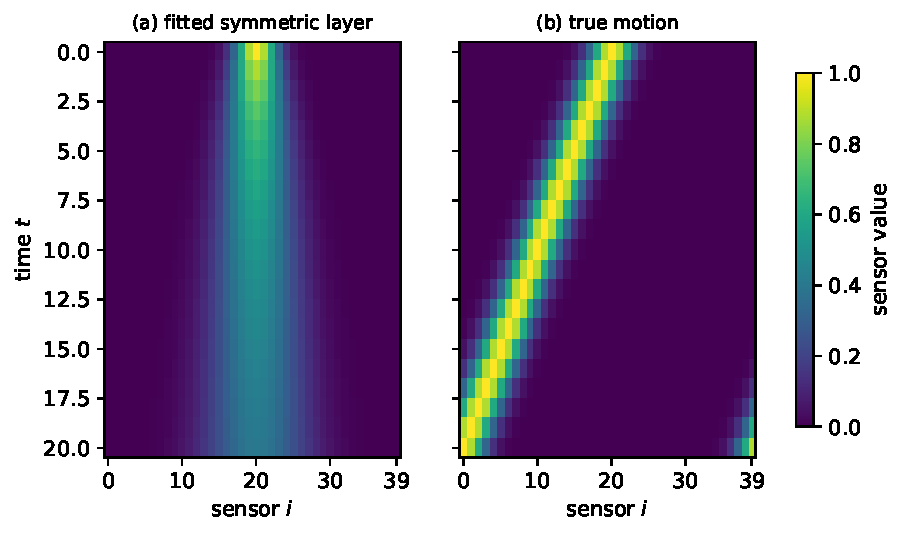
\includegraphics[width=0.8\linewidth]{fig_ring_bump.pdf}
\caption{The initial bump $x_i = e^{-(i-20)^2/8}$ ($t = 0$, top) carried 20 steps by
(a) the fitted symmetric layer of part (a)(i) and (b) the true backward-motion rule
(\texttt{np.roll(x, -1)}). Sensor index is horizontal and time increases downward; both panels
share one colour scale. The true bump translates against traffic with its shape intact (its
leading edge wraps past sensor 0 near the final steps); the fitted layer never moves it, and
instead spreads and flattens it.}
\label{fig:ringbump}
\end{figure}

The true bump translates one sensor per step against traffic, keeping its shape and height
(peak $1.000$ at every $t$, mass $5.013$ at every $t$). The fitted layer does not translate
the bump at all: it averages each sensor with its neighbours, so the bump spreads out and its
peak falls to $0.405$ by $t = 20$ while its total mass stays exactly $5.013$
(Figure~\ref{fig:ringbump}). The fitted layer conserves mass and cannot move it: diffusion,
not motion.

\section*{(b) Giving the two directions different weights}

Now give the two sides separate coefficients:
\begin{equation*}
\hat{x}_i(t+1) \;=\; a\, x_i(t) + w_{-} x_{i-1}(t) + w_{+} x_{i+1}(t).
\end{equation*}
We want the exact next snapshot for every possible input, i.e. $\hat{x}_i = x_{i+1}$ for an
arbitrary $x(t)$. That forces
\begin{equation*}
\boxed{a = 0, \qquad w_{-} = 0, \qquad w_{+} = 1,}
\end{equation*}
and the verification is: $0 \cdot x_i + 0 \cdot x_{i-1} + 1 \cdot x_{i+1} =
x_{i+1} = x_i(t+1)$ for every snapshot. The same check on 100 random snapshots gives a maximum
absolute error of exactly $0.0$. This is the whole difficulty of (a) removed in one line: the
layer is told which neighbour is ahead ($i+1$) and which is behind ($i - 1$), so the two sides
are no longer interchangeable, and a coefficient can be placed on the side that carries the
answer.

As a 1D convolution, the three entries multiplying
$[x_{i-1},\, x_i,\, x_{i+1}]$ are the kernel
\begin{equation*}
\boxed{[\,0,\; 0,\; 1\,]} .
\end{equation*}
PyTorch's \texttt{nn.Conv1d} computes cross-correlation, so no flipping is needed. The ring
boundary is handled with circular padding (\texttt{padding=1} and
\texttt{padding\_mode="circular"}), which is equivalent to index arithmetic modulo $40$ and to
\texttt{np.roll} in NumPy.

\section*{(c)(i) Equal neighbour weights, plus one step of history: backward motion}

Now the layer keeps its equal spatial weights but also gets the previous snapshot:
\begin{equation*}
\hat{x}_i(t+1) \;=\; a\, x_i(t) + b\bigl(x_{i-1}(t) + x_{i+1}(t)\bigr) + c\, x_i(t-1).
\end{equation*}
Where has the reading previously at sensor $i$ moved to at time $t$? The backward-motion rule
says $x_j(t) = x_{j+1}(t-1)$; taking $j = i - 1$ gives
\begin{equation*}
x_i(t-1) \;=\; x_{i-1}(t).
\end{equation*}
Substituting,
\begin{equation*}
\hat{x}_i(t+1)
\;=\; a\, x_i(t) + b\, x_{i-1}(t) + b\, x_{i+1}(t) + c\, x_{i-1}(t)
\;=\; a\, x_i(t) + (b + c)\, x_{i-1}(t) + b\, x_{i+1}(t).
\end{equation*}
We need this to equal $x_{i+1}(t)$ for every possible $x(t)$, which forces
\begin{equation*}
\boxed{a = 0, \qquad b = 1, \qquad c = -1,}
\end{equation*}
so the rule is $\hat{x}_i = x_{i-1}(t) + x_{i+1}(t) - x_i(t-1)$. The substitution confirms it:
since $x_i(t-1) = x_{i-1}(t)$, the rule gives $x_{i-1}(t) + x_{i+1}(t) - x_{i-1}(t) =
x_{i+1}(t) = x_i(t+1)$, exactly the true next snapshot. On 100 random snapshot pairs generated
by the backward-motion rule the maximum absolute error is $1.1 \times 10^{-16}$ (which is
floating-point noise). But the thing that is exact here: the pair $(x(t-1), x(t))$ must come from the
backward-motion rule; on arbitrary history this rule does not predict anything.

\section*{(c)(ii) The same coefficients under forward motion}

Now if we suppose instead the pattern moves forwards, $x_i(t+1) = x_{i-1}(t)$, with the previous snapshot
also produced by the same forward-motion rule. Then $x_j(t) = x_{j-1}(t-1)$, and taking
$j = i + 1$ gives
\begin{equation*}
x_i(t-1) \;=\; x_{i+1}(t).
\end{equation*}
Using the same coefficients $a = 0$, $b = 1$, $c = -1$ from (c)(i),
\begin{equation*}
\hat{x}_i(t+1)
\;=\; x_{i-1}(t) + x_{i+1}(t) - x_i(t-1)
\;=\; x_{i-1}(t) + x_{i+1}(t) - x_{i+1}(t)
\;=\; x_{i-1}(t).
\end{equation*}
And for forward motion the true next snapshot is $x_i(t+1) = x_{i-1}(t)$, so the very same
coefficients predict exactly again. On 100 random snapshot pairs generated by the forward-motion
rule the maximum absolute error is $1.1 \times 10^{-16}$. The two cases are duals of each
other: whichever neighbour the pattern came from is the one the history term cancels.

\section*{(c)(iii) Why the history breaks the symmetry}

The spatial neighbours still carry the same weight $b$, so the current snapshot alone cannot
pick a direction, exactly as in part (a). The asymmetry now lives in time. The term
$x_i(t-1)$ is equal to one of the two current neighbours, and which one depends on the
direction of motion: under backward motion the previous value is now at sensor $i - 1$
($x_i(t-1) = x_{i-1}(t)$), under forward motion it is at sensor $i + 1$ ($x_i(t-1) =
x_{i+1}(t)$). With $c = -1$ the layer subtracts exactly that neighbour, so it copies from the
one the slowdown is moving toward and nothing from the one it came from. One step of history
is enough to break the left-right tie, because it tells the layer which way the pattern has
been moving, and that is precisely the information the instantaneous, symmetric layer in part
(a) does not have.

\newpage

\taskbanner{Question 3}{Dataset Preparation and Graph Construction}

\section*{(a) Data extraction and resampling}

The raw release holds California-wide 5-minute flow for 2017--2021 but I keep only 2020 and
2021 as required. The San Diego subset is the set of PeMS District 11 sensors, which counts
716 in \texttt{ca\_meta.csv} exactly. The raw 2020 file has $366 \times 288 = 105{,}408$
five-minute steps, which become $366 \times 96 = 35{,}136$
fifteen-minute steps and the raw 2021 file has $365 \times 288 = 105{,}120$ five-minute steps,
which become $365 \times 96 = 35{,}040$ fifteen-minute steps. Both cover 8{,}600 California
sensors.

\textbf{Resampling choice.} The raw values are non-negative and integer-valued (minimum
$0.0$), and the evidence is decisive that they are interval vehicle counts rather than
average rates. The median per-sensor peak is $643$ (2020) and $650$ (2021); divided by the
sensor's own lane count this is about $161$ vehicles per lane per 5-minute step (90th
percentile $\approx 191$), i.e. roughly $2{,}000$ vehicles per hour per lane at peak. Only $8.3\%$ of positive values are multiples of $12$ (chance level)
and about $50\%$ are odd, so they are not hourly rates built from 5-minute counts. The
I-15 sensor used in part (a) peaks at $590$ over four lanes in 2021 (at 2021-09-27), about
$148$ per lane per 5-minute step. The values also top out at exactly $999$ (82 cells in 2020,
73 in 2021),
which looks like an instrument ceiling. The manual prescribes summation for interval vehicle
counts, and that is what I use: a 15-minute value is the sum of the three 5-minute readings,
using \texttt{.sum(min\_count=3)} so a window is kept only when all three readings are
present and the genuinely missing windows are
filled with $0$ afterwards. The unit is vehicles per 15 minutes, i.e. the same unit the raw
counts carry, and every later error figure in this report is in these units. This deliberately
departs from the mean-based aggregation of the official LargeST reference pipeline (a
15-minute value three times smaller); I made the choice because the manual's unit-preserving
rule applies here. Sums of integers are integers, so the integer-valued form is preserved.

\textbf{Missing values.} 4.10\% of 2020 and 6.03\% of 2021 are missing in the raw 5-minute
SD tensor, and 19 and 43 sensors are absent for the whole of each year. A window missing
even one of its three readings is treated as missing, which changes almost nothing. This
leaves about 4.1\% of 2020 and 6.0\% of 2021 missing. Those windows are filled with $0$,
following the official LargeST pipeline, and the mask of the filled windows is saved next to
the tensors (\texttt{sd\_mask\_*.npy}). In Question 4 the loss, MAE and RMSE are computed on
the valid entries only.

Genuine zero readings are rare, at about 0.3\% of valid cells. The gaps are not scattered
dropouts either. Over 90\% of gap events last an hour or less and the resample absorbs them,
but almost all missing cells sit in outages of a day or more, mostly the sensors absent for
the year. I do not interpolate the data.

This has two consequences. First, the 19 and 43 all-absent sensors become all-zero columns. I keep them
because the assignment fixes the sensor set at 716, and the mask keeps them out of the loss.
Second, about 6\% of the April--December 2021 test cells are fill, so Question 4 will report
masked test MAE and RMSE. The zero inputs of those columns still reach their neighbours
through the graph convolution; I point this out in Question 4.

\begin{figure}[htbp]
\centering
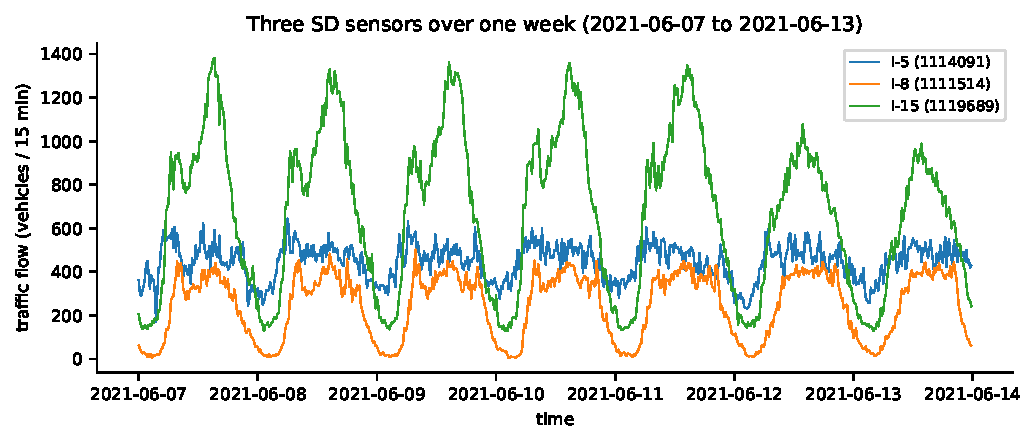
\includegraphics[width=0.95\linewidth]{fig_week_sensors.pdf}
\caption{Traffic flow at three SD sensors over one week (2021-06-07 to 2021-06-13, 672
fifteen-minute samples), in vehicles per 15-minute interval (the unit-preserving aggregate of
the raw 5-minute counts: each window is the sum of its three 5-minute readings). The I-5
sensor (1114091, N, 6 lanes) averages 445.7 (max 644), I-8 (1111514, E, 2 lanes) 247.5
(max 502), and I-15 (1119689, N, 4 lanes) 674.9 (max 1382). The sensors were picked as the
first of their highway in the dataset order; the diurnal cycle is visible in all three, with
the weekend dip on 2021-06-12/13.}
\label{fig:week-sensors}
\end{figure}

Figure~\ref{fig:week-sensors} shows one week for three sensors, one per major highway, and
the shape of a typical week: clear morning and evening peaks on weekdays, lower and flatter
over the weekend.

\section*{(b) Constructing the traffic graph}

The road-distance adjacency is provided in the release as \texttt{ca\_rn\_adj.npy}, an
$8600 \times 8600$ matrix of continuous weights in $(0, 1]$, with $1.0$ on the diagonal.
LargeST builds it from distances along the road network rather than from correlations between
the flow series. I extract the $716 \times 716$ submatrix by indexing rows and columns with
the \texttt{ID2} indices of the District-11 sensors, in the same order as the SD tensor's
columns, so sensor $i$'s row in the adjacency is sensor $i$'s column in the data. The two
orders match by construction and are asserted in the script.

\begin{table}[htbp]
\centering
\small
\begin{tabular}{@{}lr@{}}
\toprule
\textbf{quantity} & \textbf{value} \\
\midrule
nodes & 716 \\
nonzero entries, incl.\ diagonal (all 1.0) & 18{,}035 \\
nonzero entries, excluding diagonal & 17{,}319 \\
sparsity (frac.\ of 716$^2$ cells nonzero) & 3.52\% \\
degree (off-diagonal nonzeros), mean / median / min / max & 24.2 / 20 / 0 / 70 \\
sensors with zero neighbors & 8 \\
symmetric? & no \\
$\max_{i,j} |A_{ij} - A_{ji}|$ & 1.000 \\
positions where $A_{ij} \neq A_{ji}$ & 21{,}022 \\
\bottomrule
\end{tabular}
\caption{The SD road-distance adjacency submatrix. \emph{Symmetric?}\ refers to exact
equality; the two matrices differ in weights almost everywhere (see below).}
\label{tab:adj-stats}
\end{table}

\textbf{Is it symmetric? No.} The maximum absolute difference from the transpose is
$1.000$. Breaking the 17{,}319 ordered non-diagonal entries down: 13{,}608 of them sit in
pairs where both directions are nonzero (6{,}804 unordered reciprocal pairs), and the other
3{,}711 are one-directional only, which is what one-way roads produce. Even among the
reciprocal pairs the weights almost never coincide: 13{,}600 of the 13{,}608 ordered entries
disagree with their transpose, with a mean weight ratio of 4.5 and a worst case of 92. Any analysis in this
assignment that assumes a symmetric adjacency (including the default GCN normalization) would
be assuming something the data does not satisfy!

\begin{figure}[htbp]
\centering
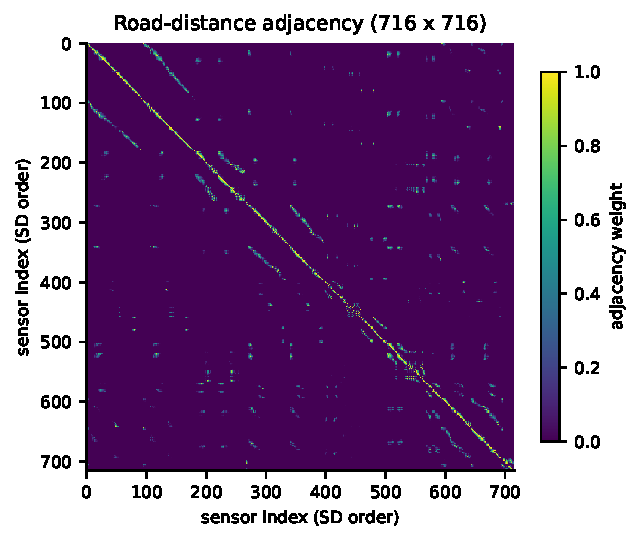
\includegraphics[width=0.62\linewidth]{fig_adjacency_heatmap.pdf}
\caption{The $716 \times 716$ road-distance adjacency. The bright diagonal is the self-loops
($A_{ii} = 1$). The near-diagonal bands are stretches of sensors on the same highway, where
successive sensors are close in road distance and their weights concentrate; the scattered
structure away from the diagonal is the rest of the network.}
\label{fig:adjacency}
\end{figure}

\begin{figure}[htbp]
\centering
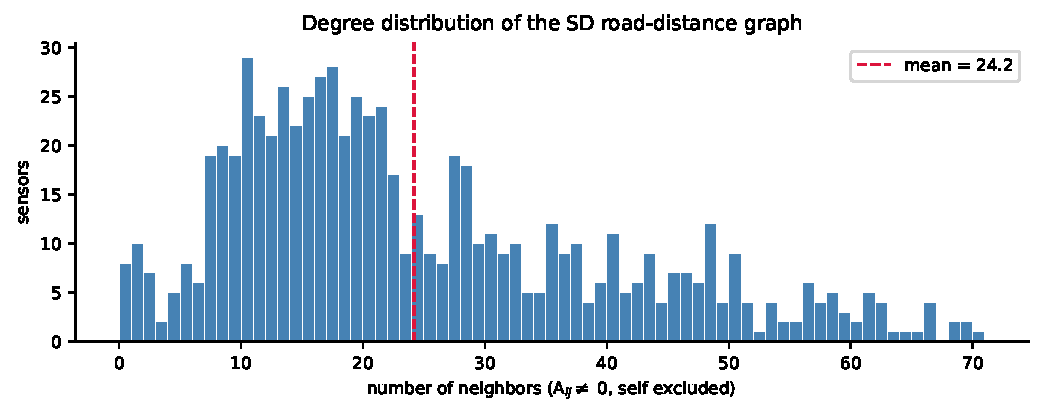
\includegraphics[width=0.75\linewidth]{fig_degree_distribution.pdf}
\caption{Neighbors per SD sensor (off-diagonal nonzeros in the adjacency), excluding
self-loops. Mean 24.2, median 20; the right tail reaches 70 and eight sensors have no
neighbor at all.}
\label{fig:degree}
\end{figure}

\textbf{What a nonzero $A_{ij}$ represents.} It is a distance-derived weight between sensor
$i$ and sensor $j$ along the road network. Diagonal entries are exactly $1.0$; off-diagonal
weights are continuous, in $(0.0100,\, 0.9999]$, with the larger ones concentrated among
consecutive sensors on the same corridor (Figure~\ref{fig:adjacency}), consistent with a
road-distance-derived kernel whose exact form is not documented in the release. 

\section*{(c) Understanding graph neighborhoods}

I take sensor 1126411 (SD row 33; I-5 northbound, direction N, ID2 6964), whose
degree of $20$ is the median degree of the SD graph. Its one-hop neighborhood, the 20 sensors
with $A_{ij} \neq 0$, is:
\begin{quote}
\footnotesize
\texttt{1114805, 1114035, 1108547, 1118707, 1117871, 1108615, 1117818, 1126426, 1114806,
1108711, 1108693, 1111514, 1113486, 1115356, 1115413, 1115432, 1115438, 1116574, 1115528,
1115517}
\end{quote}
The one-hop set is exactly the geometry of the I-5/I-8 junction. The I-8 eastbound sensor (1111514) used in
the part (a) plot is one of them, 1.4 km away. Note that the set spans both carriageways of
both freeways: near this junction the support of the adjacency is essentially
direction-blind, and the asymmetry lives in the weights rather than in the zero pattern. Its
two-hop neighborhood (at most two edges away, and excluding the node itself) has $73$
members, of which $53$ are not in the one-hop set; adding one more graph layer reaches them.

\textbf{Why neighboring sensors help predict this sensor.} Traffic does not change
independently sensor by sensor; congestion propagates along the corridor at vehicle speeds. A
neighbor just upstream sees a slowdown some minutes before it arrives at 1126411, and a
neighbor just downstream sees it some minutes after it leaves, and both of those readings are
in the same direction of motion. The eight-timestamp, two-hour input window gives the layer
the temporal
dimension (how fast and how far the pattern is travelling); the graph gives it the spatial one
(where the same pattern is right now). A model restricted to 1126411's own history cannot see
the wave coming; a model with its one-hop neighborhood can.

\textbf{One-hop vs two-hop aggregation.} One-hop aggregation lets a node use its direct
neighbors once; a single graph convolution layer does exactly that, and each additional layer
reaches one more edge. Two-hop aggregation reaches the upstream-of-upstream sensors, which
matters when a slowdown originates far enough up the corridor that it has not reached the
direct neighbors yet, and it lets the model distinguish ``a wave two segments back, moving
toward me'' from a local fluctuation. The cost is depth: each extra layer re-mixes the node's
own signal with more distant sources, so the influence of far nodes is diluted and less
reliable, and the layer count, not the data, decides how much spatial context the model
trusts.

\textbf{Could using too many graph convolution layers hurt? Yes.} Three things! (i) Over-smoothing: stack enough graph layers and every node's representation
converges to the same vector, at which point the forecast ignores the sensor entirely; this is
the graph analogue of the symmetric-diffusion failure in Question 2, where the fitted layer
spread the bump instead of moving it. (ii) Dilution: on a graph with mean degree $24$, a few
layers mix in orders of magnitude more sources than any sensor can usefully integrate, and
the model spends its capacity denoising its own neighbors. (iii) Cost and miscalibration:
with attention or gates absent, deeper layers add compute without adding information the
problem needs, and the asymmetric, one-way structure of this graph means long paths can route
information in directions that are not physically meaningful.

\newpage

\taskbanner{Question 4}{Spatio-Temporal Traffic Forecasting}

All code is in \texttt{q4/code/stgcn.py}; results are in \texttt{q4/results/}
(\texttt{stgcn\_stgnn\_s0.json}, \texttt{stgcn\_temporal\_s0.json}).

\section*{(a) Preparing forecasting windows}

For each prediction time $t$, the model sees the previous eight 15-minute steps and
predicts the next four:
\begin{equation*}
X_t = [x_{t-7}, \dots, x_t], \qquad Y_t = [x_{t+1}, \dots, x_{t+4}], \qquad x_t \in \mathbb{R}^{716 \times 1}.
\end{equation*}
Chronological splits, as required:
\begin{table}[htbp]
\centering
\small
\begin{tabular}{@{}lrrr@{}}
\toprule
\textbf{split} & \textbf{period} & \textbf{steps} & \textbf{windows} \\
\midrule
training & Jan--Dec 2020 & 35{,}136 & 35{,}125 \\
validation & Jan--Mar 2021 & 8{,}640 & 8{,}629 \\
testing & Apr--Dec 2021 & 26{,}400 & 26{,}389 \\
\bottomrule
\end{tabular}
\caption{The chronological splits and, from them, the number of forecasting windows per
split. No window crosses a boundary: windows are formed inside each split independently.
Both years are at 15-minute resolution, and every window spans eight observed steps and
four predicted ones.}
\label{tab:splits}
\end{table}

The normalisation statistics are computed from the training split only, over the valid
(non-filled) entries: mean $607.17$, standard deviation $483.35$. The same transform is
applied to the validation and test splits unchanged. Evaluations are reported in the
original units (vehicles per 15 minutes) by scaling back. The zero-filled windows are in
the tensor, but the loss and the reported metrics are computed only on the valid entries,
following the Question 3 decision; about $6\%$ of the test cells are fill and are excluded.

\section*{(b) Implementing the forecasting architecture}

The model has the three required components.

\textbf{Temporal encoder.} Two \texttt{Conv1d} layers ($1 \to 32$ and $32 \to 32$, kernel
size 3, padding 1) with a ReLU after each, applied per sensor. The feature at the last
position is taken, so the encoder produces $Z \in \mathbb{R}^{B \times N \times 32}$.

\textbf{Spatial graph convolution.} $H = \mathrm{ReLU}(\hat{A} Z W_g)$ with $W_g \in
\mathbb{R}^{32 \times 32}$ (no bias). $\hat{A}$ is a row-normalised version of the provided
road-distance adjacency: $\hat{A} = D_{\mathrm{out}}^{-1} A$, where $D_{\mathrm{out}}$ is
the diagonal matrix of row sums of $A$. The adjacency is not symmetric, so the usual
$D^{-1/2}(A+I)D^{-1/2}$ normalization is not applicable; the row-normalized form is the
standard choice for directed graphs and matches the manual's one-hop definition
$N(i) = \{j : A_{ij} \neq 0\}$. The unit diagonal is a self-loop, so the eight sensors with
no off-diagonal neighbor get $\hat{A}_{ii} = 1$ and are well-defined.

\textbf{Forecast head.} A small MLP: Linear$(32 \to 32)$, ReLU, Linear$(32 \to 4)$, applied
per sensor, producing the next four 15-minute values.

\textbf{Training.} Masked L1 loss (MAE) in normalized units; Adam (learning rate $10^{-3}$),
batch size 128, 20 epochs, seed 0, no tuning. 5{,}444 trainable parameters; 78.98\,s on a GPU PC (NVIDIA GeForce RTX 5060 Ti), 3.9\,s per epoch.

\begin{table}[htbp]
\centering
\footnotesize
\begin{tabular}{@{}lrrrrrr@{}}
\toprule
\textbf{model} & \textbf{val MAE} & \textbf{val RMSE} & \textbf{test MAE} & \textbf{test RMSE} & \textbf{params} & \textbf{time} \\
\midrule
STGNN (fixed road-distance adjacency) & 133.0 & 208.0 & 147.7 & 224.6 & 5{,}444 & 79\,s \\
Temporal-only & 69.6 & 109.7 & 75.7 & 117.0 & 4{,}420 & 75\,s \\
\bottomrule
\end{tabular}
\caption{Validation and test MAE and RMSE in original units (vehicles per 15 minutes), seed
0. Both models share the temporal encoder and the forecast head; the STGNN adds one graph
convolution layer. The temporal-only model is the better model by a wide margin.}
\label{tab:q4-results}
\end{table}

\begin{figure}[htbp]
\centering
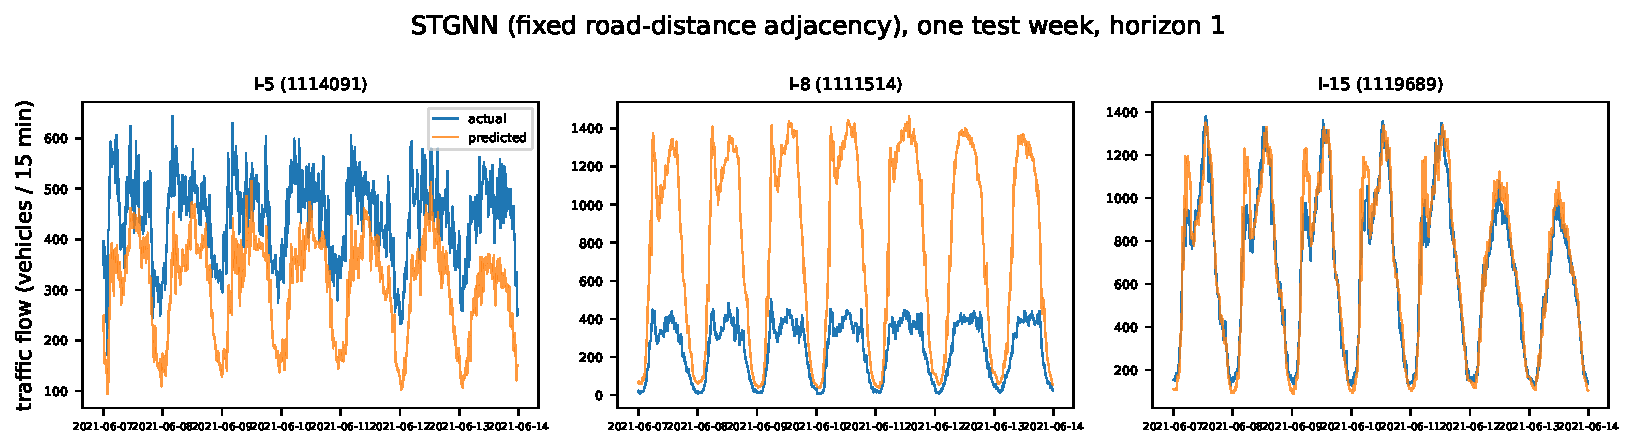
\includegraphics[width=0.98\linewidth]{fig_q4_predictions.pdf}
\caption{Horizon-1 predictions on one test week (2021-06-07 to 2021-06-13) for the fixed
road-distance model; the I-8 panel shows the failure analyzed in part (c).}
\label{fig:q4-pred}
\end{figure}

\section*{(c) Temporal-only baseline}

The baseline uses the same temporal encoder and forecast head but no graph convolution,
with identical data, preprocessing, hyperparameters and seed. It has 4{,}420 parameters and
trains in 74.8\,s (3.7\,s per epoch). The comparison (Table~\ref{tab:q4-results}) is direct:
same protocol, same budget, one seed, final-epoch weights.

The spatial layer does not help here. It hurts, and in one case it hurts badly. Per-sensor
test MAE for the three report sensors: the temporal-only model is 67.2, 38.4 and 66.7 for
I-5, I-8 and I-15; the graph model is 143.1, 515.7 and 101.3. The I-8 failure is not a
dead-neighbour failure. Dropping the 43 sensors absent for all of 2021 from the graph and
retraining leaves the test MAE at 147.5 and I-8 at 561.2, so the present-vs-absent layout
is not the cause. The cause is the aggregation itself. Under $\hat{A} = D_{\mathrm{out}}^{-1} A$,
sensor 1111514 keeps only 6.6\% of its weight on itself; the neighbour-weighted mean flow of
its neighbours is about 532 against its own about 237. That level mismatch is what it shares
with the sensors that fail: per-sensor test MAE correlates with the mismatch at a Spearman
rank of 0.67 (and with the dead-neighbour share at only 0.20). A 50/50 self-vs-neighbour
split in the same adjacency ($\hat{A}' = 0.5 I + 0.5 \hat{A}$) recovers most of the ground:
test MAE falls to 79.8 and I-8 to 45.2.

Three reasons the fixed graph hurts at this scale, in descending order of importance.
First, self-dilution: the manual's $H = \mathrm{ReLU}(\hat{A} Z W_g)$ replaces the encoder's
output with an about-$94\%$-neighbour-weighted mean rather than adding to it, so the head
reads a representation dominated by other sensors' dynamics and almost ignoring this sensor's
own. Second, no residual path: nothing carries the sensor's own features around the graph
layer, and it is needed exactly when the neighbour-weighted mean is a bad model of this
sensor. Third, relevance: this adjacency is built from road-network distance, and it links
sensors for which the physical connection is close but the traffic pattern is weakly related;
without a learned weight or a gate it cannot tell them apart at this budget.
The caveat that matters is that this is one seed, one lightweight model, twenty epochs, and
a single fixed adjacency; it is evidence about {this} particular design, not about graphs in
general.

\begin{table}[htbp]
\centering
\footnotesize
\begin{tabular}{@{}lccc@{}}
\toprule
\textbf{variant} & \textbf{val MAE} & \textbf{test MAE} & \textbf{I-8 test MAE} \\
\midrule
fixed (default) & 133.0 & 147.7 & 515.7 \\
fixed (50\% self, $\hat{A}' = 0.5 I + 0.5 \hat{A}$) & 73.7 & 79.8 & 45.2 \\
fixed (43 dead sensors removed) & 133.1 & 147.5 & 561.2 \\
\bottomrule
\end{tabular}
\caption{Two quick ablations of the aggregation structure behind the I-8 failure. The
50/50 self-vs-neighbour split recovers most of the ground; removing the dead sensors does
not.}
\label{tab:ablation}
\end{table}

\newpage


\taskbanner{Question 5}{Fixed versus Learnable Adjacency Matrices}

The fixed graph hurts, so this question asks whether learning the graph does better. I
implement the three adjacency variants with one code path: the same temporal encoder,
forecasting head, dataset splits, and training protocol as in Question 4 (masked L1 loss,
Adam at $10^{-3}$, batch size 128, 20 epochs, seed 0), so any difference is attributable
primarily to graph construction.

\section*{(a) Fixed adjacency}

The fixed adjacency is the $716 \times 716$ road-distance submatrix from Question 3, used
unchanged throughout training. As the graph is not symmetric, I do not apply the symmetric
$D^{-1/2}(A+I)D^{-1/2}$ normalization; instead $\hat{A} = D_{\mathrm{out}}^{-1} A$, the row-normalised
form chosen in Question 4, which is well-defined for every row including the eight sensors
with no off-diagonal neighbor (their row sum is 1, from the unit diagonal). The graph is a
fixed buffer in the model; it never changes during training. The protocol reruns
differ slightly from the first run (val 133.07 / 208.43, test 147.80 / 224.92); I did not
isolate the cause. The numbers reported throughout are from the latest full rerun
(val 132.95 / 207.98, test 147.67 / 224.55).
The fixed-adjacency model is the one that
broke down on the I-8 sensor in Question 4, and the ablation in that section
(Table~\ref{tab:ablation}) shows the failure is a self-dilution of the aggregation,
not the poisoned neighbours.

\section*{(b) Learnable adjacency}

Instead of the physical graph, the model learns one. I introduce two trainable node
embedding matrices $E_1, E_2 \in \mathbb{R}^{716 \times 32}$, initialized from a Gaussian
with standard deviation $0.05$, and construct $A_{\mathrm{adaptive}} = \mathrm{Softmax}(\mathrm{ReLU}(E_1 E_2^{\top}))$,
with the softmax applied row-wise (each row sums to 1). The embeddings are updated by
backpropagation alongside the rest of the model. I do not sparsify: at 716 nodes the dense
matrix is cheap, the softmax is already row-stochastic, and top-k sparsification would force
a choice about whether to apply it before or after normalization that I would rather not
make. Unlike the fixed adjacency, this graph can connect sensors that are not physically
adjacent. The model is trained with the same protocol as in Question 4; the only change is
where the aggregation weights come from.

\begin{table}[htbp]
\centering
\footnotesize
\begin{tabular}{@{}lrrrrrr@{}}
\toprule
\textbf{model} & \textbf{val MAE} & \textbf{val RMSE} & \textbf{test MAE} & \textbf{test RMSE} & \textbf{params} & \textbf{time} \\
\midrule
STGNN, fixed adjacency & 133.0 & 208.0 & 147.7 & 224.6 & 5{,}444 & 79\,s \\
STGNN, adaptive adjacency & \textbf{64.89} & \textbf{103.47} & \textbf{75.19} & \textbf{115.78} & 51{,}268 & 81\,s \\
STGNN, hybrid adjacency & 73.95 & 119.69 & 83.47 & 127.91 & 51{,}268 & 81\,s \\
(reference) temporal-only & 69.61 & 109.69 & 75.73 & 117.01 & 4{,}420 & 75\,s \\
\bottomrule
\end{tabular}
\caption{Validation and test MAE and RMSE in original units (vehicles per 15 minutes),
seed 0, for the three adjacency variants and, for reference, the temporal-only model from
Question 4. Train time is the full run on the Lab PC (RTX 5060 Ti); the adaptive and hybrid
models add 45{,}824 embedding parameters ($2 \times 716 \times 32$) to the 5{,}444 shared
ones. Different rows use the same temporal encoder, head, splits and protocol, so the
differences are attributable primarily to graph construction.}
\label{tab:q5-results}
\end{table}

The adaptive adjacency is the best of the graph models, and it edges the temporal-only
baseline slightly on val (64.89 vs 69.61) and on test RMSE (115.78 vs 117.01); on test MAE
they are close enough to call a tie (75.19 vs 75.73). It beats the fixed graph by a factor
of two. The learned graph is visualised in
Figure~\ref{fig:adaptive-adj}: it is denser than the road map, but concentrated rather than diffuse. Of its entries only 55{,}200 ($10.8\%$) are above $10^{-3}$ (against 17{,}319
total for the physical graph), the median row puts 56.5\% of its mass on its 10 largest
neighbours, and a diagonal component survives (the largest single diagonal row weight is
0.856). Across nodes, only
12.7\% of the ten largest learned neighbours are physically adjacent in the road graph. The learned adjacency actually
assigns \emph{more} weight, not less, to the sensors that are dead in 2021 (9.5\% of its
total mass, against 5.9\% for the row-normalised physical graph, and 44.2\% against 26.4\%
at the I-8 sensor), so the improvement is not the model learning to avoid dead neighbours;
the physical structure itself was the wrong inductive bias for this task and this budget. The caveat is
capacity: the adaptive and hybrid models carry 46k more parameters than the fixed-graph one,
and the cleanest control against a pure capacity explanation is the hybrid, which has the
same 51{,}268 parameters and is clearly worse on test MAE (83.47 vs 75.19) — though both
large models are in the same range as the temporal-only baseline.

\begin{figure}[htbp]
\centering
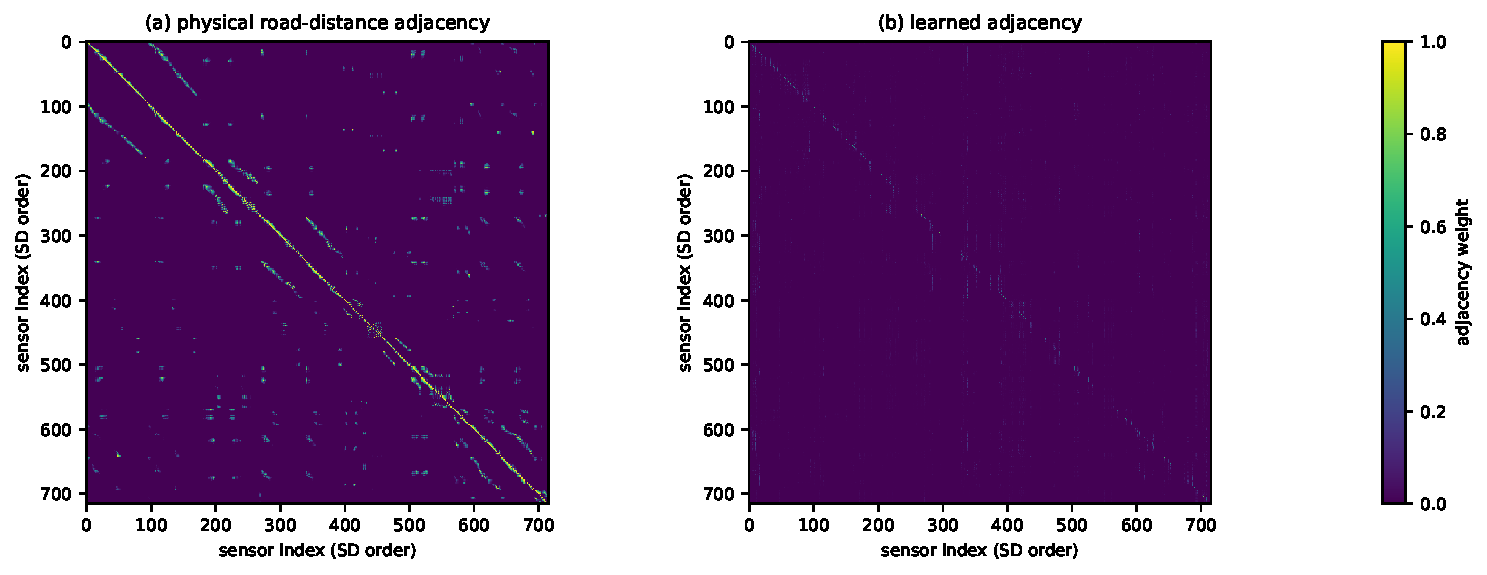
\includegraphics[width=0.98\linewidth]{fig_adjacency_learnt.pdf}
\caption{(a) The physical road-distance adjacency, for reference. (b) The learned
adjacency. Most of its mass is off the diagonal, and its links are mostly different from
the physical ones.}
\label{fig:adaptive-adj}
\end{figure}

\section*{(c) Hybrid adjacency}

The hybrid graph is $A_{\mathrm{hybrid}} = \alpha A_{\mathrm{fixed}} + (1-\alpha)
A_{\mathrm{adaptive}}$ with $\alpha = 0.5$ fixed, not learned (keeping the comparison clean).
Both terms are row-stochastic by construction ($A_{\mathrm{fixed}}$ is the row-normalised
physical graph and $A_{\mathrm{adaptive}}$ has row-wise softmax), so the combination is a
convex average and gradients flow through the learned half exactly as before.

The hybrid model is second best. It is much better than the fixed one (val 73.95 / 119.69,
test 83.47 / 127.91) and clearly worse than the adaptive one: the fixed half reintroduces
some of the mismatch that makes the Q4 graph fail, at the same parameter count as the
adaptive model. The results are not subtle: fixed is catastrophic, hybrid is a drag,
adaptive is best of the graph models (val 64.89, test 75.19 / 115.78 RMSE) and only narrowly
beats or ties the temporal-only baseline (75.73 / 117.01). Learning the graph is strictly
better than asserting one at this scale and budget; adding the spatial layer at all
contributes almost nothing over the plain temporal model on test.

Two caveats though. This is one seed, 20 epochs and a lightweight model, and the adaptive
graph is concentrated rather than a discovered sparse-structured graph. And on this data and budget
the margins between adaptive, hybrid and fixed are large; I have not tested whether they
survive multiple training seeds or a different model size.

\taskbanner{Question 6}{Experimental Analysis and Interpretation}

This question pulls the Question 4 and 5 models together and asks what their numbers
actually say. Every comparison below uses the same test period (April--December 2021), the
same protocol, and the same metrics as the earlier questions. All code and result files are
under \texttt{q6/} (\texttt{q6/code/q6\_analysis.py}, \texttt{q6/results/q6\_analysis.json},
and the figures).

\section*{(a) Forecasting comparison}

\begin{table}[htbp]
\centering
\small
\begin{tabular}{@{}lrrrr@{}}
\toprule
\textbf{model} & \textbf{adjacency} & \textbf{MAE} & \textbf{RMSE} & \textbf{training time} \\
\midrule
Temporal-only & none & 75.7 & 117.0 & 75\,s \\
STGNN & fixed (road-distance) & 147.7 & 224.6 & 79\,s \\
STGNN & adaptive (learned) & \textbf{75.2} & \textbf{115.8} & 81\,s \\
STGNN & hybrid (fixed + learned) & 83.5 & 127.9 & 81\,s \\
\bottomrule
\end{tabular}
\caption{Test-set MAE and RMSE in original units (vehicles per 15 minutes), seed 0. These
are the same numbers reported in Questions 4 and 5 (the fixed-adjacency row is from the latest
rerun, which differs by about 0.1 MAE from the first run). Validation metrics are in Tables 4 and 5; train
times are wall-clock on the Lab PC (RTX 5060 Ti).}
\label{tab:q6-results}
\end{table}

The three sensors used throughout the report behave as expected in the comparison (Figure~\ref{fig:pred_actual}): the
adaptive model tracks all three well, including I-8, where the fixed-graph model failed to follow the actual series.

\begin{figure}[htbp]
\centering
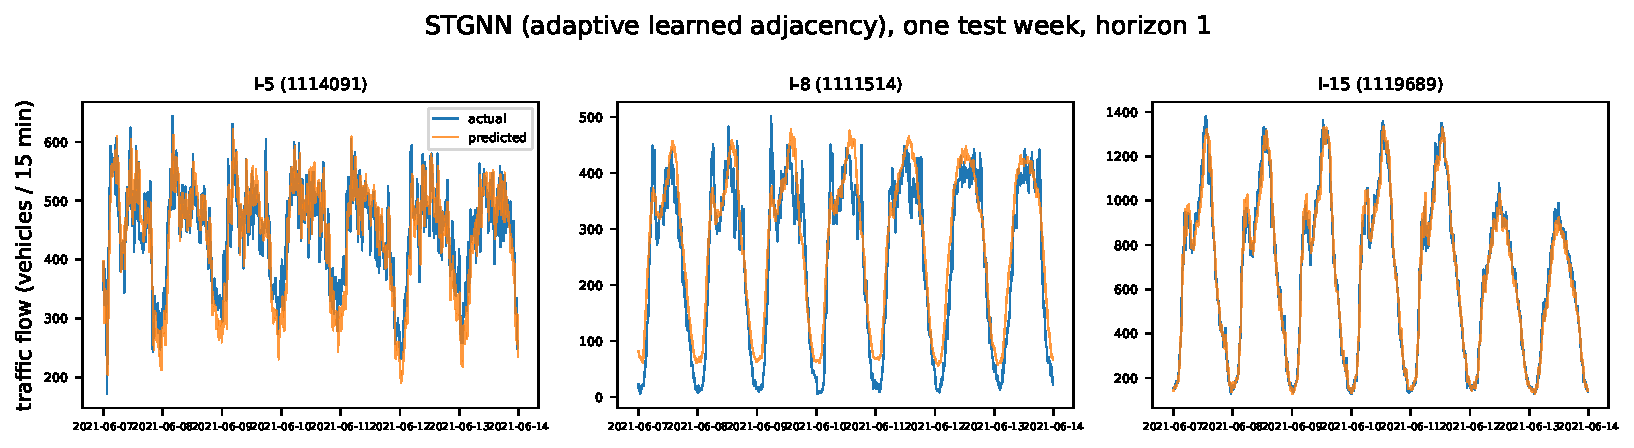
\includegraphics[width=0.98\linewidth]{fig_pred_actual.pdf}
\caption{Actual vs predicted horizon-1 traffic flow over one test week
(2021-06-07 to 2021-06-13) for the three report sensors, from the adaptive-adjacency
model. Predictions track the actual series closely at all three sensors, including
I-8, which the fixed-adjacency model failed badly.}
\label{fig:pred_actual}
\end{figure}

\section*{(b) Graph structure analysis}

\textbf{1. Are the strongest learned connections also in the physical graph?} No. Only
27.4\% of the learned graph's strongest neighbours (its top-1 per node) are physically
adjacent; the overlap falls to 16.1\% at top-5, 12.7\% at top-10 and 9.3\% at top-20.
Conversely, only 5.3\% of physical adjacency survives into the learned top-10 and 7.7\%
into the top-20. The learned graph is denser than the physical one but not close to full:
55{,}200 of its entries are above $10^{-3}$ ($10.8\%$ of off-diagonal cells, against the
physical graph's 17{,}319 nonzero entries), and the median row puts 56.5\% of its mass on
its 10 largest entries.

\textbf{2. Do learned connections tend to occur between geographically nearby sensors?}
Mostly no. The learned top-10 connections average 22.99\,km apart, against 5.89\,km for the
physical top-10 and 27.09\,km for random pairs: they are barely closer than a random pair.
Their distinguishing feature is corridor structure, not proximity: 36.6\% of the learned
top-10 fall in the same highway corridor (against 70.5\% for the physical graph), so the
model leans on freeway co-movement, not on the road layout.

\textbf{3. Can the learned graph capture dependencies absent from the physical graph?}
Yes, by construction it is mostly not the physical graph: 87.3\% of the learned top-10 links
are absent from the physical adjacency, and the flow correlation of the learned top-10 is
$0.892$ (against $0.860$ for the physical top-10). The learned graph can and does link
sensors that are distant on the road network yet move together. What that tells us is
informative only under an assumption that the training traffic statistics persist; the
graph is a statistical fit, not a physical map.

\textbf{4. Why might a learned adjacency perform better or worse than a fixed one?}
Better when the data has co-movement structure that the road network does not encode; worse
when the learned graph overfits the training regime, when the encoder can use it to memorize
rather than to generalize, or when the physical graph's prior regularizes an otherwise
unconstrained fit. Here the fixed graph actively hurt most because of its aggregation
structure (sensor 1111514 keeps only 6.6\% of its weight on itself), not because of the
dead neighbours; the learned graph spreads its mass over many neighbours, which
functionally raises the self-share without ever asking for it. Relative to the
temporal-only baseline (75.73 test MAE), both large-observation-budget models add almost
nothing (adaptive 75.19, hybrid 83.47): the flexible graph does not beat the encoder by
much on this budget, and the hybrid's 8-point gap points at the fixed component being a
drag, not at the learned component being a lift. Whether the learned links are truly
informative on out-of-distribution traffic (a crash rerouting traffic onto a different road)
is untested here.

\section*{(c) Critical discussion}

\textbf{Does a lower forecasting error mean the learned graph represents actual road
connectivity?} No. It means the test-set numbers are lower. The learned graph does not
respect directionality, does not decay with distance, is nearly dense, and is mostly
disjoint from the road map; calling it connectivity would be interpreting a regression's
fitted weights as a physical fact. The correct reading is that traffic at a sensor is
predicted better when the model is allowed to pool from co-moving sensors rather than only
from adjacent ones. It is a useful statistical summary, not a map.

\textbf{Why might a hybrid graph outperform either fixed or adaptive alone?} In general the
hybrid can dominate both when the two carry complementary signal that neither has alone: the
fixed graph as a prior stabilises the adaptive one when data is scarce, and the adaptive
one extends coverage where the physical grid is sparse or wrong. It can also interpolate
between over- and under-constrained regimes. In this run the hybrid (0.5/0.5) did not beat
the pure adaptive model: I-8 MAE is 65.9 for the hybrid against 48.1 for the adaptive one
and 515.7 for the fixed one, so the fixed component drags a little but not catastrophically;
most of the damage is gone by halving its weight. A smaller α might match or beat adaptive though
I did not tune it.

\textbf{What are the limitations of using a static graph?} Traffic dependencies are not
stationary in time. Corridors flip their correlation sign between rush hour and late-night,
weekday and weekend traffic loads reorganise around different bottlenecks, and an incident
(or even rain) reroutes volume onto different roads within minutes. A static graph averages
all of those regimes into one symmetric-tending matrix that cannot switch with conditions;
it cannot represent the sudden emergence of a new dominant corridor dependency, and it will
not adjust its routing when one corridor goes from helpful to irrelevant in an hour. A
time-conditioned or regime-switching graph, or attention conditioned on recent observations,
is the natural extension. Static here also applies to the training regime: the learned graph
fits this dataset's habitual co-movement and carries no mechanism for noticing that a
sensor has gone silent or that a freeway has changed its direction pattern.

\taskbanner{Question 7}{Reproducibility and Reporting}

Everything in this report is reproducible from the repository. The repository itself
holds code, the result JSONs and the figures; the heavy artifacts (the raw LargeST
release, the processed SD tensors, the masks, the trained weights) stay on the Lab PC and
are regenerable with the commands listed in the README. This section collects the
implementation choices and maps each required item to where it stands.

\begin{table}[htbp]
\centering
\small
\begin{tabular}{@{}p{1.2in}p{5.6in}@{}}
\toprule
\textbf{component} & \textbf{setting} \\
\midrule
input and target & 8 observed 15-minute steps, 4 predicted, $X_t = [x_{t-7} \dots x_t]$, $Y_t = [x_{t+1} \dots x_{t+4}]$, $x_t \in \mathbb{R}^{716 \times 1}$ \\
splits & train Jan--Dec 2020 (35{,}125 windows); val Jan--Mar 2021 (8{,}629); test Apr--Dec 2021 (26{,}389); no window crosses a boundary \\
preprocessing & 5-minute intervals summed to 15 minutes (the manual's counts rule); all-missing and partial windows filled with $0$; the mask of filled windows is saved \\
normalisation & training split only, over valid (non-filled) entries: mean 607.17, std 483.35, applied unchanged to val and test \\
model & per-sensor temporal \texttt{Conv1d} encoder ($1 \!\to\! 32 \!\to\! 32$, kernel 3, padding 1, ReLU); one directed graph convolution $H = \mathrm{ReLU}(\hat{A} Z W_g)$, $\hat{A} = D_{\mathrm{out}}^{-1} A$; MLP head ($32 \to \mathrm{ReLU} \to 4$) \\
adjacencies & fixed (road-distance, row-normalised, unchanged in training); adaptive ($\mathrm{softmax}(\mathrm{ReLU}(E_1 E_2^{\top}))$, row-wise); hybrid ($0.5$ fixed $+$ $0.5$ adaptive) \\
loss and metrics & masked L1 (MAE) in normalised units; MAE and RMSE reported in original units on the valid entries only \\
optimizer & Adam, learning rate $10^{-3}$, batch 128, 20 epochs; seed 0 for all scripts \\
parameters & temporal-only: 4{,}420; STGNN fixed: 5{,}444; STGNN adaptive/hybrid: 51{,}268 \\
hardware & NVIDIA GeForce RTX 5060 Ti (16 GB); measured 79\,s / 75\,s / 81\,s / 81\,s for the four models \\
\bottomrule
\end{tabular}
\caption{Implementation choices and training configuration, identical for every model in
Questions 4--6 unless noted.}
\label{tab:config}
\end{table}

\begin{table}[htbp]
\centering
\small
\begin{tabular}{@{}p{2.2in}p{4.6in}@{}}
\toprule
\textbf{required item} & \textbf{where it lives} \\
\midrule
source code with instructions & \texttt{q1}--\texttt{q6} directories; the README's Reproducing section lists the exact commands \\
model hyperparameters, epochs, random seed & Table~\ref{tab:config}; the code constants in \texttt{q4/code/stgcn.py}; the per-model JSONs in \texttt{q4/results/} and \texttt{q5/results/} \\
final comparison table & Table~\ref{tab:q6-results} (and Tables~\ref{tab:q4-results}, \ref{tab:q5-results}) \\
at least one adjacency visualization & Figures~\ref{fig:adjacency}, \ref{fig:degree} and \ref{fig:adaptive-adj} \\
predicted vs actual plots & Figures~\ref{fig:q4-pred} and \ref{fig:pred_actual} (plus the week traces in Figure~\ref{fig:week-sensors}) \\
hardware specifications and measured training times & Table~\ref{tab:config}; Tables~\ref{tab:q4-results}, \ref{tab:q5-results} and \ref{tab:q6-results}; the per-model JSONs \\
\bottomrule
\end{tabular}
\caption{The Question 7 checklist mapped to its locations in this submission.}
\label{tab:q7checklist}
\end{table}

\newpage



\section*{Generative AI Declaration}

In accordance with the course policy on generative AI, I declare that I used an AI
coding and research assistant (Claude Code) throughout this assignment. I decide what to
study, what to test and what to claim; the assistant writes and runs the code, produces
the figures and tables from saved results, and drafts the report text under my direction.
The analysis and every claim are mine.

\textbf{What the AI did.} It wrote every code file in this repository: the Q1
verification (the 164 triples), the q2 ring-road experiment, q3's data pipeline on the
GPU PC, the STGNN and temporal-only baseline of Q4, the three adjacency variants of q5,
and the q6 analyses. It ran every experiment, saved the logs and JSONs, and generated the
figures and tables from them.

\textbf{What I did.} I supplied the mathematics behind Questions 1 and 2 (the
base-$(K+1)$ encoding and the aggregation table; the least-squares fit, the convolution
kernel, and the history-based coefficients for the ring road). I designed every experiment: the valid-entry-only
normalization, the masked-loss protocol and the one shared split across models rule.

\end{document}
